\section*{Merge-Sort}

$T(n) = 2*T(n/2) + n$

\textbf{Worst-, Best- und Average-Case:} 

$\mathcal{O}(n*log(n))$, selten Worst-Case $\mathcal{O}(n^2)$

Zusätzlicher Speicher von $\mathcal{O}(n)$

\begin{minted}[breaklines]{java}
private void sort(int[] a, int beg, int end) {

    if (end - beg > 1) {
        int m = (beg + end) >>> 1;
        sort(a, beg, m);
        sort(a, m, end);
        merge(a, beg, m, end);
    }
}

private void merge(int[] a, int beg, int m, int end) {
    int[] b = new int[end - beg];

    int i = 0, j = beg, k = m;
    while (j < m && k < end) {
        if (a[j] <= a[k]) b[i++] = a[j++];
        else b[i++] = a[k++];
    }
    while (j < m) {
        b[i++] = a[j++];
    }
    while (i > 0) {
        --i;
        a[beg + i] = b[i];
    }
}
\end{minted}

\subsection*{Merge Inplace}

\begin{minted}[breaklines]{java}
private void sort(int[] a, int beg, int m, int end) {

	int j = beg, k = m;
	while(j != k && k != end) {
		if(a[j] <= a[k]){
			j++;
		} else {
			int temp = a[k];
			for(int i = k; i > j; i--){
				a[i-1] = a[i];
			}
			a[j] = temp;
			k++;
			j++;
		}
	}
 }
\end{minted}

\subsection*{Merge Halber-Speicher}

\begin{minted}[breaklines]{java}
private void merge(int[] a, int beg, int m, int end) {
	int[] b = new int[m-beg];
	for(int i = beg; i < m; i++) {b[i-beg] = a[i];}
	int i = beg, j = 0, k = m;
	while (0 < (m - beg) || k < end) {
		if(b[j] < a[k]){
			a[i] = b[j]; i++; j++;
		} else {
			a[i] = a[k]; i++; j++;
		}	
	}
	while(j < (m-beg)){
		a[i] = b[j]; i++; j++;
	}
}
\end{minted}

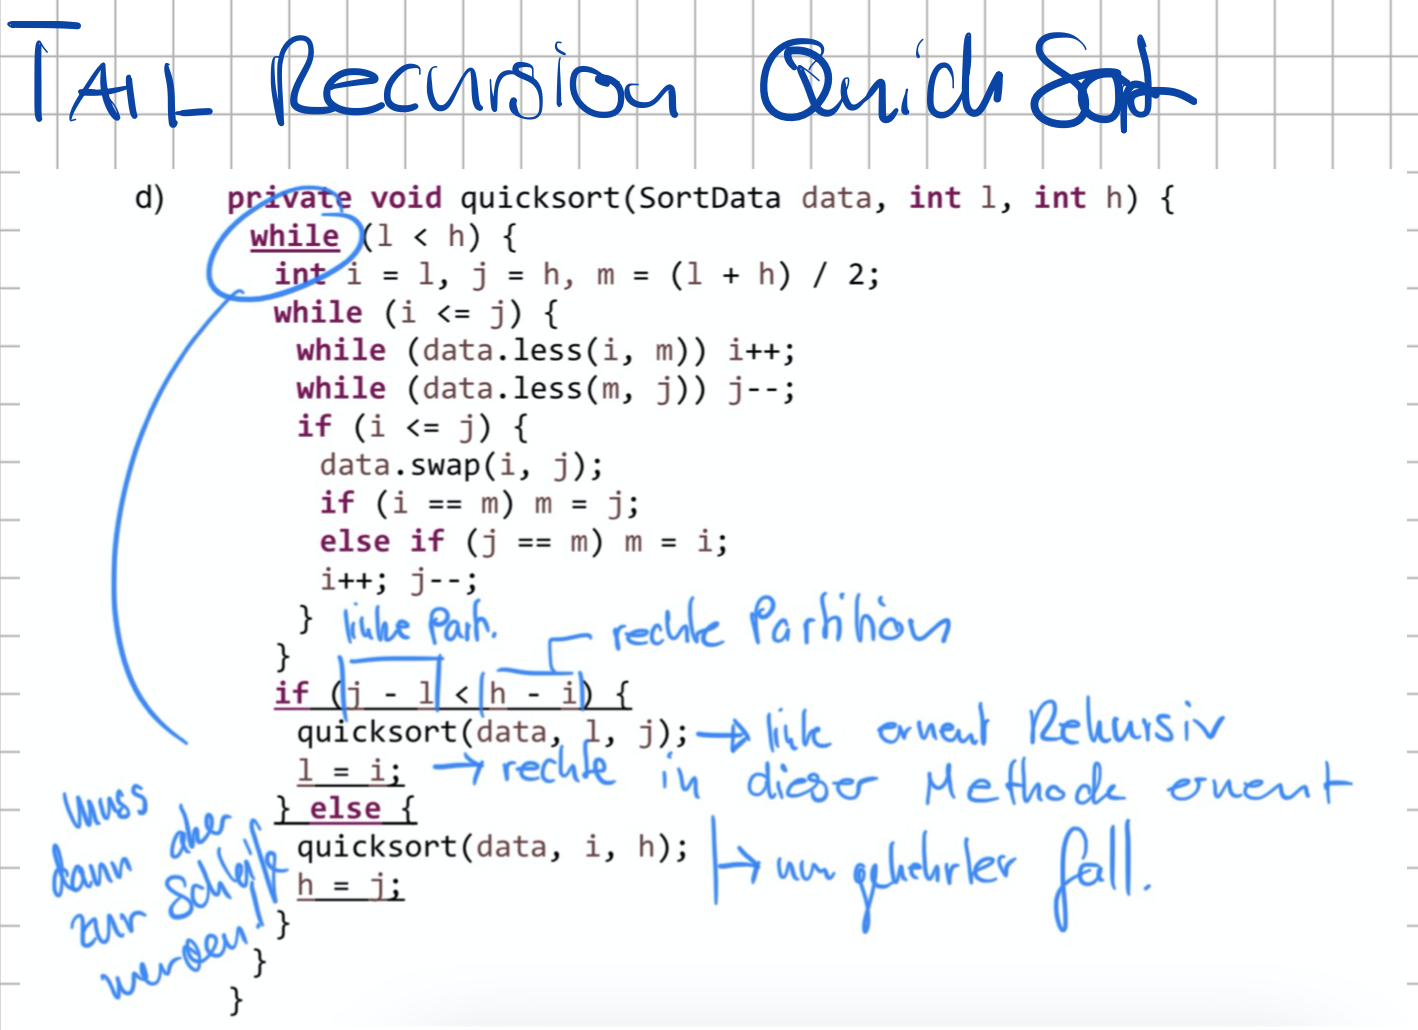
\includegraphics[width=\linewidth]{images/tailrecursion}
